% --- CHAPTER 4: IMPLEMENTATION ---
\section{Implementation}
\label{sec:implementation}

This chapter describes the technological stack and programmatic patterns used to convert the abstract design of AdriaBOX into a working software prototype. The codebase is implemented entirely in Python, using a modular architecture to enforce clean boundaries between core network utilities, data transfer engines, and control services. On the client side, architectural responsibilities are structuralized around a central \texttt{AdriaClient} object acting as a Facade interface that seamlessly orchestrates the control-plane operations of \texttt{AdriaHTTPClient} and the low-level data-plane transfer mechanisms handled by \texttt{AdriaTransferManager}.

\subsection{Network and Application Protocols}
AdriaBOX utilizes a hybrid networking model to optimize performance and separate tasks within the infrastructure:
\begin{itemize}
    \item \textbf{Control Plane Communication (HTTP/1.1):} All client interactions with the metadata controller rely on synchronous HTTP REST APIs. This traffic is handled via the Python \texttt{requests} library on the client side, using a persistent \texttt{requests.Session()} object to maintain and reuse underlying connection contexts efficiently. The utilization of persistent connection pools limits the operational TCP handshake overhead, minimizing connection latency during structural control operations.
    \item \textbf{Data Plane Communication (Raw TCP Sockets):} High-throughput binary streaming between client transfer components and storage workers uses raw, low-level TCP/IP sockets via Python's native \texttt{socket} library. Sockets are initialized with explicit timeout constraints to prevent resource leaks from broken pipes or network drops. By operating on raw octet streams, the data plane completely bypasses the computational text-parsing overhead characteristic of higher-level application layer frameworks.
\end{itemize}

\subsection{In-Transit Data and Wire Layout Serialization}
Data encapsulation and wire serialization layout decisions depend on the operational context of the payload:
\begin{itemize}
    \item \textbf{Control Structures and Metadata:} Inter-component operational exchange payloads (such as cluster layouts, upload/download plans, and system responses) are serialized into standard JSON text strings. This data layout supports flexible schema alterations while keeping parsing overhead low across REST endpoints.
    \item \textbf{Network Framing Primitives:} To construct custom binary stream headers over raw TCP, the system utilizes Python's native \texttt{struct} library. Packing directives enforce strict data serialization sizes and layout alignments:
    \begin{itemize}
        \item Format token \texttt{>I} is applied to serialize metadata block capacities into an unsigned 32-bit integer (4 bytes) using Big-Endian formatting, aligning with standard Network Byte Order rules.
        \item String paths and parameter payloads are packed into variable-length binary arrays using standard UTF-8 text encoding.
    \end{itemize}
\end{itemize}
This precise binary layout prevents message fragmentation anomalies across socket boundaries, ensuring that any receiver can deterministically partition incoming framing packages before extracting volatile data payloads.

\subsection{Database Persistence and Relational Query Strategy}
The metadata server tracks global cluster state and user accounts using Python's native \texttt{sqlite3} module. The system maps directory entries and user records to an embedded relational SQLite database (\texttt{metadata.db}). 

To ensure clean, readable access, connections are configured with the custom attribute \texttt{conn.row\_factory = sqlite3.Row}. This converts standard relational row collections into structured object maps, allowing fields to be accessed directly by column name. 

Data updates leverage standard SQL transactions managed by context handlers (\texttt{with sqlite3.connect() as conn}). This architecture ensures ACID properties for cluster state updates, preventing corrupt or partial metadata mappings during concurrent file tracking requests. The system handles transaction isolation natively, mitigating deadlocks or dirty reads during high-concurrency storage node updates.

\subsection{Authentication Matrix and Session Token Tracking}
Tenant authentication relies on a stateless, token-based framework using the \texttt{PyJWT} library. When a user logs in, the metadata controller validates their identity against salted password hashes. 

Upon validation, the server generates a cryptographically signed JSON Web Token (JWT) embedded with the tenant's user ID, username, assigned system role, and a strict 24-hour expiration timestamp (\texttt{exp}). The signature is secured with a private cluster key using the HMAC-SHA256 algorithm. 

The client command-line interface caches this token locally within an isolated configuration structure. The local persistence layer handles the active token safely within user-space directories, ensuring that concurrent client instances on the same host station isolate their respective cryptographic states natively without data pollution. The token is systematically appended as a bearer string to the authorization headers of all subsequent API calls, allowing the control plane to validate tenant requests securely without maintaining server-side session state.

\subsection{Authorization and Multi-Tenant Access Control}
Access controls are enforced on the server using an Aspect-Oriented Programming (AOP) approach. The system wraps target API endpoints inside a central validation decorator method denominated \texttt{\_auth\_and\_route()}. This middleware wrapper extracts incoming token headers, validates the cryptographic signature, checks the expiration timestamp, and passes the validated user context to the underlying business logic. 

Authorization boundaries implement a hybrid Model-Based and Role-Based Access Control (RBAC) strategy:
\begin{itemize}
    \item \textbf{Standard Users:} Restricted by ownership filters. SQL query statements include strict tenant boundaries (e.g., matching the user context ID against file owner records) to prevent accounts from accessing or enumerating data assets outside their authorized scope.
    \item \textbf{System Administrators:} Authorized by checking for the \texttt{admin} role string within the token payload. Validated administrative sessions can run unrestricted database queries to monitor overall cluster telemetry or evict user accounts.
\end{itemize}

\subsection{Technical Implementation Modules and Package Dependencies}
The implementation layout and component modularity are structured according to the package schematic shown in \Cref{fig:implementation_packages}.

\begin{figure}[htbp]
    \centering
    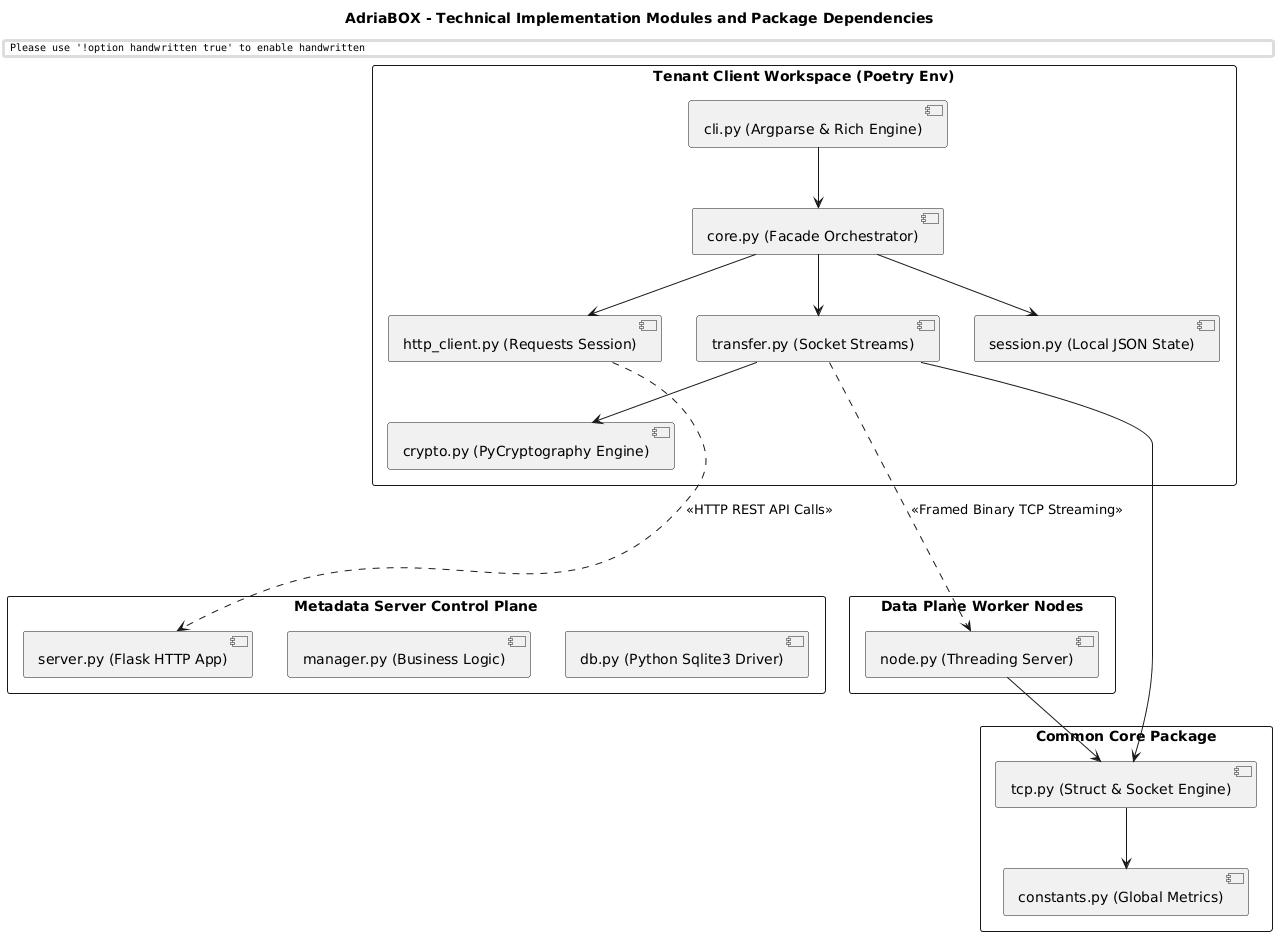
\includegraphics[width=\textwidth]{plantuml/4.1-implementation-packages.png}
    \caption{AdriaBOX Technical Implementation Modules and Source File Dependencies.}
    \label{fig:implementation_packages}
\end{figure}

The software artifact utilizes specific open-source libraries to meet its security and user interface requirements:
\begin{itemize}
    \item \textbf{Flask Framework:} Operates as the foundation for the control server, routing network traffic to dedicated controller classes and processing incoming JSON metadata blocks via micro-routing modules.
    \item \textbf{Werkzeug Security Library:} Manages secure credential persistence. User passwords are never saved in plaintext; instead, they are converted into robust cryptographic hashes using the standard \texttt{pbkdf2:sha256} algorithm combined with random salt strings.
    \item \textbf{PyCryptography Component:} Provides the low-level mathematical engine for the client workspace, using advanced symmetric ciphers (\texttt{AES-256-CTR}) and key derivation primitives (\texttt{PBKDF2HMAC} with a 100,000-iteration counter) to execute Zero-Knowledge security routines.
    \item \textbf{Rich UI Framework:} Drives the terminal user interface engine. It processes raw directory arrays and system reports to render clean, interactive data tables and color-coded panels, improving usability while keeping the client lightweight.
    \item \textbf{Poetry Environment Coordinator:} Manages project dependencies and execution environments, defining precise version boundaries for internal modules to guarantee stable and reproducible deployments across different host systems.
\end{itemize}

\subsection{Operational Interaction of the Technology Stack}
To illustrate how these independent open-source components integrate dynamically during system execution, the programmatic data flow between libraries is mapped sequentially within \Cref{fig:technological_flow}.

\begin{figure}[htbp]
    \centering
    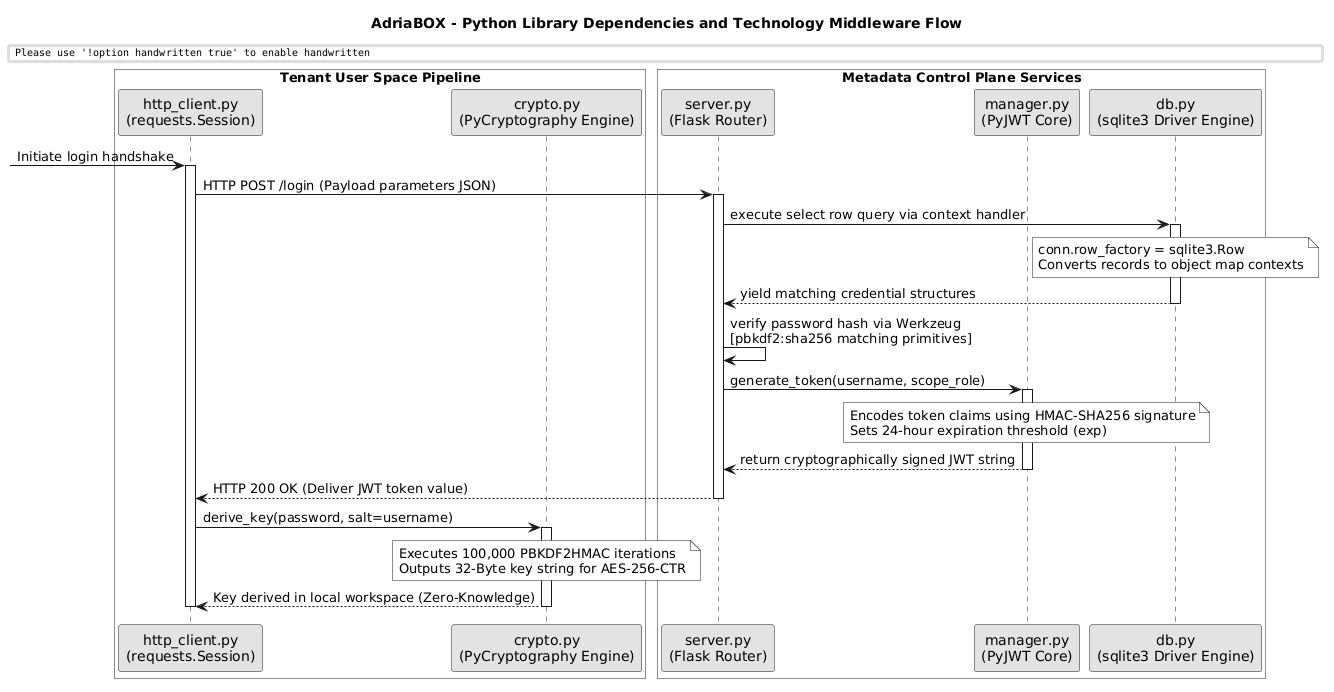
\includegraphics[width=0.95\textwidth]{plantuml/4.2-technological-flow.png}
    \caption{AdriaBOX Inter-Component Software Library Dependency and Operational Middleware Execution Lifecycle.}
    \label{fig:technological_flow}
\end{figure}

This mapping visualizes the execution pipeline during a standard session initialization. Incoming HTTP parameter strings map through the \texttt{Flask} routing layer into the relational database context. The \texttt{sqlite3} engine packages row properties using column identifiers, allowing the server to retrieve verification parameters securely. 

Credential evaluation is offloaded to \texttt{Werkzeug} hashing blocks, and session tracking is initialized via \texttt{PyJWT} primitives to compile a signed authorization bearer token. Simultaneously, in complete isolation from the network plane, the local client workspace targets the \texttt{PyCryptography} primitives to execute the rigorous 100,000 iteration key derivation loops, sealing the client cryptographic context before data plane transactions begin.

\subsection{Low-Level Programmatic Flow and Simulation Isolation Mechanics}
To establish an uncompromised evaluation framework for the distributed architecture, specific technical mechanics are implemented within the codebase components to enforce multi-client segregation and bounded memory streaming.

\subsubsection{The Upload Conflict and Stream Pipelining Logic}
When an execution routine invokes an upload operation within \texttt{AdriaClient}, the system enforces a strict state evaluation sequence. The method first intercepts the directory context via an explicit call to \texttt{list\_files()} to inspect the current catalog state. If a filename collision is detected, the runtime halts execution to prompt an interactive overwrite authorization. Upon user confirmation, a clean purge command is propagated via \texttt{self.rm()} to forcefully scrub obsolete metadata entries and orphan chunks, eliminating ghost block accumulation before fetching a new upload allocation plan from the Master orchestration core.

Once the plan payload is retrieved from the control endpoints, high-throughput streaming is offloaded to \texttt{AdriaTransferManager.upload\_file\_chunks()}. This routine handles file data isolation by wrapping operations inside an explicit context manager:

\begin{lstlisting}[language=Python]
with open(local_filepath, "rb") as source:
    for chunk in plan_chunks:
        source.seek(chunk["offset"])
        # Instantiate localized socket sender and stream bytes...
\end{lstlisting}

The transfer engine moves the file cursor to the calculated byte offset, bypassing heavy block memory replication. For each individual block sequence, the system instantiates a localized \texttt{ChunkStreamSender} instance using target TCP parameters. Crucially, the unique tracking attribute \texttt{file\_id} is systematically stringified into a dedicated \texttt{session\_id} variable and injected directly into the transmission pipeline. This identifier colors downstream octet packets, enabling backend worker thread contexts to map incoming byte sequences to an explicit orchestration context without loading un-segmented assets into volatile memory.

\subsubsection{POSIX User-Space Workspace Emulation Isolation}
Although AdriaBOX is designed to run over discrete physical stations distributed across a network domain, testing multi-client operational boundaries requires an environment capable of executing multiple active workflows concurrently. Multi-client session isolation is handled natively via the \texttt{SessionManager} constructor layout:

\begin{lstlisting}[language=Python]
def __init__(self, session_file="session.json"):
    home_dir = os.path.expanduser("~")
    self.session_file = os.path.join(home_dir, ".adriabox", session_file)
    os.makedirs(os.path.dirname(self.session_file), exist_ok=True)
\end{lstlisting}

By invoking the native \texttt{os.path.expanduser("\textasciitilde")} method, the local runtime dynamically binds the state storage directory to the current POSIX home folder inside the active file system block. Within the Docker-based emulated testbed, each client node container inherits an isolated, independent root partition directory. Consequently, when concurrent users execute commands simultaneously, the underlying JSON session records, Bearer JWT credentials, and active symmetric encryption key parameters are written to segregated local paths. This architecture completely prevents cross-tenant credential leakage or session overwrite collisions across workstations, validating production-grade trust boundaries on a single host.

\subsubsection{Zero-Knowledge Cryptographic Execution Primitives}
Symmetric security metrics are implemented using deterministic stretching and inline byte mutations inside the client execution perimeters. The method \texttt{CryptoManager.derive\_key()} seals the user context via a rigorous multi-layered key derivation pipeline:

\begin{lstlisting}[language=Python]
salt = username.encode('utf-8').ljust(16, b'\0')[:16]
kdf = PBKDF2HMAC(
    algorithm=hashes.SHA256(),
    length=32,
    salt=salt,
    iterations=100000,
    backend=default_backend()
)
\end{lstlisting}

The system enforces key isolation by applying the unique tenant \texttt{username} string as a deterministic salt primitive, padding the byte sequence to exactly 16 bytes using a trailing zero-byte truncation mask (\texttt{.ljust(16, b'\textbackslash{}0')[:16]}). This configuration eliminates identical key derivations for users sharing duplicate passwords. The key derivation function executes 100,000 stretching iterations using the cryptographic primitive \texttt{SHA256}, locking the computation inside local user-space memory pages.

When streaming data blocks, \texttt{CryptoManager.get\_stream\_cipher()} extracts a distinct 16-byte Initialization Vector (Nonce) for each data chunk by passing the explicit \texttt{chunk\_filename} string through an independent hashing primitive:

\begin{lstlisting}[language=Python]
digest = hashes.Hash(hashes.SHA256(), backend=default_backend())
digest.update(chunk_filename.encode('utf-8'))
nonce = digest.finalize()[:16]
\end{lstlisting}

This structural mechanism ensures that identical plaintext payloads split across separate file components yield entirely unique ciphertext octet streams on the wire. The resulting \texttt{Cipher} configuration instantiates an Advanced Encryption Standard (\texttt{AES}) mechanism running in Counter (\texttt{CTR}) mode. CTR mode virtualizes block boundaries, computing a mathematical keystream on the fly that executes in-place XOR bit modifications on the 4KB transmission staging buffer, eliminating memory padding delays and ensuring absolute isolation from cloud data-plane components.